\documentclass{article}
\usepackage{tikz}
\usepackage{array}
\usepackage{calc}
\usepackage{setspace}
\usepackage{amsmath}
\usepackage{xspace}
\usepackage{color}
\usepackage{pgfplots}
\usetikzlibrary{shapes.geometric, arrows}

\tikzstyle{startstop} = [rectangle, rounded corners, minimum width=3cm, minimum height=1cm,text centered, draw=black, fill=red!30]
\tikzstyle{io} = [trapezium, trapezium left angle=70, trapezium right angle=110, minimum width=3cm, minimum height=1cm, text centered, draw=black, fill=blue!30, text width = 2cm]
\tikzstyle{process} = [rectangle, minimum width=3cm, minimum height=1cm, text centered, draw=black, fill=orange!30, text width = 2cm]
\tikzstyle{decision} = [diamond, minimum width=3cm, minimum height=1cm, text centered, draw=black, fill=green!30, text width = 2cm]
\tikzstyle{arrow} = [thick,->,>=stealth]
\pgfplotsset{width=10cm,compat=1.9}

\newcommand\mTW{1.5cm}
\newcommand{\TODO}[1] {{\color{red}\textbf{TODO: #1}}}
\newcommand{\citeme}{\TODO{[Citation Needed]}}

\begin{document}
\title{XSgen}
\date{January, 25, 2017}
\author{Flanagan, Robert \and Scopatz, Anthony}
\maketitle
\onehalfspacing

\section{Introduction}
Reactor simulation is an essential part of nuclear fuel cycle modeling. Modeling strategies
may be categorized in three ways: low, medium, and high fidelity. Each of these modeling
paradigms provides different benefits to a fuel cycle simulation but comes with tradeoffs to
either accuracy, computational effort, or both.

Low fidelity models are those models that include limited to no physical computations at run time.
This class of modeling works best for systems that have fixed behaviors. For example, a reactor
during steady state operation may be modeled sufficiently accurately with a low fidelity model.
Such models are often refered to as \emph{recipe reactors}. A recipe represents a predefined
nuclide vector. Recipe reactors use fixed pairs of input and output recipes to
match fresh and spent
fuel respectively. This lookup table strategy is a computationally efficient mechanism to
represent reactor operation. Alternatively, low fidelity models may include interpolation
techniques to build libraries on the fly. For example, interpolating between recipes for
3\% U-235 enriched fuel, and 4\% enriched fuel might be used to obtain a 3.5\% enriched
fuel recipe.
However, interpolating in this manner fails to directly capture any of the physical changes
that might happen to the core by switching from either 3\% or 4\% enriched fuel to a 3.5\% fuel.

Medium fidelity models are those that include physics calculations, but fall short of
full neutron transport or multiphysics calculations. These models typically require
pre-built datasets which are constructed from the results of higher fidelity models.
Medium fidelity models synthesize these pre-built datasets with reasonablly fast physics
algorthims ($<1$ minute execution time). This combination of well structured data and
quick solvers allows for a significatly higher degree of modularity, flexibility, and accuracy
for medium fidelity models over their low fidelity counterparts. Additionally, their average
execution time is orders of magnitude lower than full neutron transport and multiphysics
calculations. Examples of medium fidelity reactor models are Class\cite{class}
and Bright-lite\cite{brightlite,flanagan}.

High fidelity models are performed using neutronics calculations, Bateman
equation\cite{Bateman} solvers, or other coupled multiphysics algorithms. These models tend
to require information about on the complete reactor design in order to specify and execute.
Additionally, due to their higher accuracy, these models require a proportionally heavy amount
of computation to complete. An example of a high fidelity reactor model is the
MCNP\cite{mcnp5monte} burn card which couples Monte Carlo neutron transport with a depletion
calculator.

Medium fidelity models provide useful middle road between accuracy and computational effort
for nuclear fuel cycle simulators. However, they may vary greatly in the mechanisms and
techniques that they employ. Bright-lite uses a fluence based neutron balance approach to
determine the behavior of the reactor. It also includes optional physics behaviors, such as
disadvantage factors, batch physics, and fuel blending. Alternitavely, Class uses a set of
reactor input and output recipes and recursive neural networks\citeme to dynamically determine
reactor behavior. To understand how these different modeling choices impact a fuel cycle
scenario it is important for the models to have same fundemental information basis.
For example, when comparing medium fidelity reactor models, one-group cross sections
must be the same.

At present, each medium fidelity model uses its own method for generating input datasets.
This implies that any methodlogical comparison between would be (at least partially) invalid
because each model starts with distinct inputs. Thus, any difference in their outputs
could be attributable to differences in inputs and any similarities in outputs could be
happenstance. Therefore, only an analysis that uses the same baseline datasets
is useable for teasing out differnces that arrise purely from methodology.

This paper discusses a method which generates datasets usable by medium fidelity reactor models.
The authors term this method XSgen and a concrete implementation of this method is available
in the cooresponding BSD-licensed XSgen software package.

XSgen couples a neutron transport code with a depletion solver to automate the generation of
medium fidelity reactor model datasets. XSgen uses OpenMC\citeme as neutron transport.
A one thousand group logarithimically spaced flux is extracted from OpenMC. This flux is
measured in the fuel region of supplied reactor geometry. This flux is fed into a cross
section collapser to generate one-group or multi-group cross sections. This operation is
performed by PyNE\cite{pyne}, the nuclear engineering toolkit. Finally, either the
one-group or multi-group cross sections are coupled to a depletion solver. Currently, this
role is satisfied by ORIGEN v2.2\cite{origen2}, which requires one-group cross-sections.

The XSgen method is capable of providing all of the inputs that medium fidelity reactor models
may use: time dependent one- or multi-group cross sections, transmutation matricies,
burnup rates, neutron production rates, and destruction rates.
XSgen stores the specified data which it generates a single database.
From here, medium fidelity reactor models are able extract the information they need to
derive a new dataset for use in a fuel cycle simulation.

XSgen can also be used to set up more accurate comparisons between low fidelity recipe reactor
models and medium fidelity reactor model types. This is made possible because XSgen may also
simulate a fuel bundle well past its effective lifetime in the core. The data generated by an
XSgen run of this type contains enough information to build out an estimate of core composition
at discharge using reactor batch physics discussed later below.

\TODO{Add a paragraph about the sections to come. \S 1 discusses...}

\section{XSgen Workflow}
The main line of the XSgen workflow couples three primary tools: neutron transport via OpenMC,
cross section collapse via PyNE, and depletion ORIGEN v2.2. The first step is the simulation
of the reactor core using a Monte Carlo neutron transport simulation. The primary result of
this is a highly resolved flux spectrum. This spectrum is then collapsed with a standard
cross section database and converted into a suite of one-group cross sections for a reactor
at time step $t$ [days] after the reactor has started up. These one-group cross sections are
then used by a depletion solver to compute the burnup, neutron production rate, neutron
destruction rate, and transmutation matrices. The value of $t$ is set by the user when XSgen
is executed. The composition of the material at the end of the time step is then submitted
back to the neutron transport solver as input. This process is repeated until the maximum time
step specified is reached. The XSgen workflow is displayed in Figure \ref{fig:flow}.

\begin{figure}\center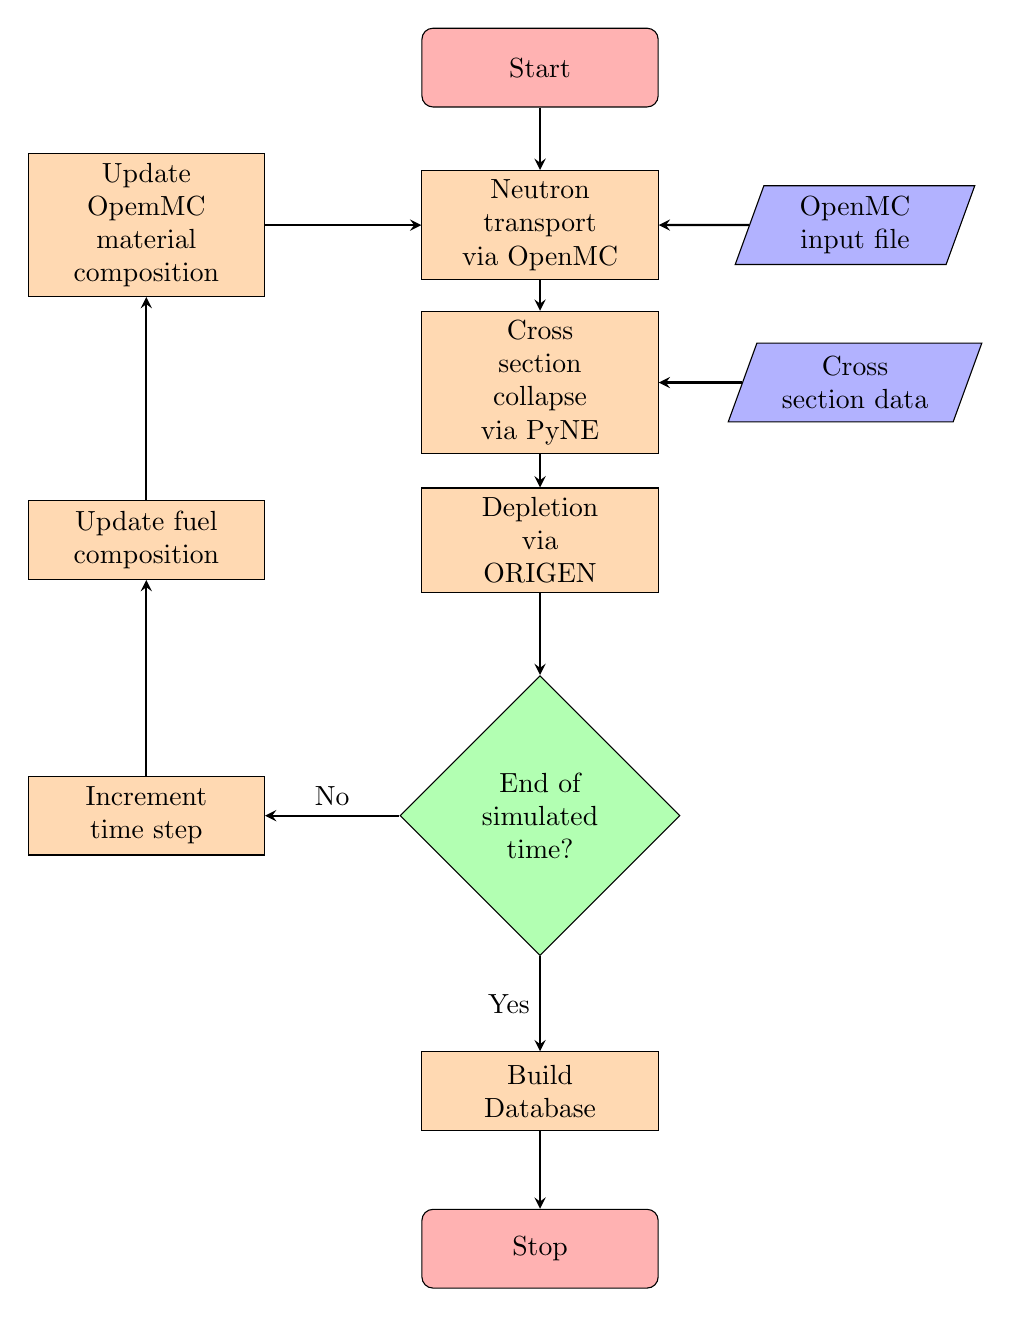
\begin{tikzpicture}[node distance=2cm]
\node (start) [startstop] {Start};
\node (openmc) [process, below of = start]{Neutron transport via OpenMC};
\node (omcinput) [io, right of = openmc, xshift = 2cm]{OpenMC input file};
\node (omcupdate) [process, left of = openmc, xshift = -3cm]{Update OpemMC material composition};
\node (pyne) [process, below of = openmc]{Cross section collapse via PyNE};
\node (pynexs) [io, right of = pyne, xshift = 2cm]{Cross section data};
\node (origen22) [process, below of = pyne]{Depletion via\\ORIGEN};
\node (compupdate) [process, left of = origen22, xshift = -3cm]{Update fuel composition};
\node (timecheck) [decision, below of = origen22, yshift = -1.5cm]{End of simulated time?};
\node (timeinc) [process, left of = timecheck, xshift = -3cm]{Increment time step};
\node (brightlite) [process, below of = timecheck, yshift = -1.5cm]{Build Database};
\node (stop) [startstop, below of = brightlite] {Stop};
\draw [arrow] (start) -- (openmc);
\draw [arrow] (omcinput) -- (openmc);
\draw [arrow] (omcupdate) -- (openmc);
\draw [arrow] (openmc) -- (pyne);
\draw [arrow] (pynexs) -- (pyne);
\draw [arrow] (pyne) -- (origen22);
\draw [arrow] (origen22) -- (timecheck);
\draw [arrow] (compupdate) -- (omcupdate);
\draw [arrow] (timeinc) -- (compupdate);
\draw [arrow] (timecheck) -- node[anchor=south]{No}(timeinc);
\draw [arrow] (timecheck) -- node[anchor=east]{Yes}(brightlite);
\draw [arrow] (brightlite) -- (stop);
\end{tikzpicture}
\caption{Flow chat of the XSgen process for building medium fidelity reactor databases.}
\label{fig:flow}
\end{figure}

\subsection{OpenMC}
OpenMC was used as the reference neutron transport calculator for modeling reactors.
It was chosen due to its availablity (it is BSD licensed), its ability to quickly perform
reactor oriented calculations\cite{serpentvmonte}, and it capability to compute scattering
kernels. Currently, XSgen only obtains the group flux values from OpenMC. It extracts
these for each timestep.

Input templates for OpenMC can be specified in the XSgen run control file.
New templates may be constructed for a reactor design by creating a new input file for OpenMC
and templating it according to a set of field variabless that XSgen provides.
XSgen also provides standard templates representing pressurized water reactor (PWR)
and fast reactor (FR) lattices. More standard templates may be added to XSgen in the future.

\subsection{PyNE}
PyNE is used to perform the group collapse
from cross section databases down to the one-group or multi-group cross sections.
PyNE is capable of reading in cross section data from both ACE\cite{ace} and ENDF\cite{endf}
datasets. It is able to synthesize cross section data - that may exist with
many different energy grids - down to a single, standard energy group structure specified
by the user.

The algorithm PyNE uses for collaspsing cross sections is tailored to efficiently collapsing
the same group structure over many different data sets.
It operates by first constructing a partial energy matrix (PEM). This matrix maps a higher
resolution group structure to a lower resolution group structure. It does this by determining
the contribution of each of the higher resolution energy groups into the lower resolution
energy groups using a weighted sum. A PEM is only applicable for the transformation it is
originally designed for. For example, a PEM that transforms a 10 group system into a
1 group system can not be used to transform a 20 group system into a 1 group system.
The calculations required to generate a PEM can be computationally expensive
and therefore are only performed if a new group structure is added to the system.

Here, $\vec{\phi_h}$ represents the high resolution group fluxes for $H$ energy groups with
a group structured defined by $E_h$ bin boundaries. Likewise, $\vec{\phi_g}$ represents
the collapsed flux with $G$ groups and $E_g$ bin boundaries. The partial energy
matrix $P$ is defined by the relations seen in Equation \ref{pem-relations}.
Equation \ref{pem-relations} assumes that all energies are monotonically decreasing, namely
that $E_{g+1} \le E_{g} \forall g\in G$ and $E_{h+1} \le E_{h} \forall h\in H$.
\begin{equation}
\label{pem-relations}
P_{g,h} = \left\{
\begin{array}{ll}
    0 & : E_{g} > E_{h} \\
    0 & : E_{g-1} < E_{h+1} \\
    \left(\frac{E_h - E_g}{E_h - E_{h+1}}\right) & : (E_{g} \le E_h) \, \& \, (E_{g} \ge E_{h+1}) \\
    \left(\frac{E_{g-1} - E_{h+1}}{E_h - E_{h+1}}\right) & : (E_{g-1} \le E_h) \, \& \, (E_{g} \le E_{h+1}) \\
    1 & : (E_{g} \le E_{h+1}) \, \& \, (E_{g-1} \ge E_{h}) \\
\end{array}
\right.
\end{equation}
Once $P$ is obtained, collapsing a dataset (such as group fluxes or group constants) from $H$
groups into $G$ groups requires only taking the dot product of the PEM
by the data set. Equation \ref{phi-h-to-g} demonstrates this for group fluxes and Equation
\ref{sig-h-to-g} shows this transition for group constants.
\begin{equation}
\label{phi-h-to-g}
\vec{\phi_g} = P \cdot \vec{\phi_h}
\end{equation}
\begin{equation}
\label{sig-h-to-g}
\vec{\sigma_g} = P \cdot \vec{\sigma_h}
\end{equation}
Importantly, the PEM $P$ may be reused as many times as necessary and the dot product in
Equations \ref{phi-h-to-g} \& \ref{sig-h-to-g} is relatively cheap computationally.

The above PEM expressions are usable when groupwise cross sections are already available.
However, when only ENDF or ACE continous energy data is available for a nuclide, these pointwise
cross sections must be collapsed to groupwise versions.
In Equation \ref{pointwise-collapse}, $E_j$ represents the energy of a pointwise cross section in the data set,
$\sigma(E_j)$ represents the cross section at energy $E_j$, and $\sigma_{r,g}^i$ represents a
groupwise cross section for $i^\mathrm{th}$ nuclide and the $r^\mathrm{th}$ reaction channel.
\begin{equation}
\label{pointwise-collapse}
\sigma_{r,g}^i = \frac{1}{2} \frac{\sum_{E_j\ge E_{g+1}}^{E_j\le E_g}
                                   \left(\sigma(E_j)+\sigma(E_{j+1})\right)
                                   \left(E_{j+1}-E_{j}\right)}
                                  {E_g-E_{g+1}}
\end{equation}
Equation \ref{pointwise-collapse} amounts to a trapezoidal integration weighted by the
energy width of the group. From here, one-group cross sections may be obtained using the PEM
matrix from above. Note that in Equation \ref{pointwise-pem}, $\phi$ represents the total
flux ($\phi=\sum\phi_g$).
\begin{equation}
\label{pointwise-pem}
\sigma_{r}^i=\frac{P \cdot (\overrightarrow{\sigma_{r,g}^i \phi_g})}{\phi}
\end{equation}
Here $\sigma_{r}^i$ represents the one-group cross section of the $r^\mathrm{th}$ reaction
channel for the $i^\mathrm{th}$ nuclide and $\overrightarrow{\sigma_{r,g}^i \phi_g}$ is the
elementwise multplication of the group constants and the group fluxes.
This process is repeated for all nuclides and reaction channels. The resultant one-group
cross section dataset is used to construct a custom ORIGEN v2.2 TAPE9 file\cite{origen2}.

Pyne will also allow the user to incorperate the effects of self-shielding into XSgen. It does this by building an energy dependent function of weights for each isotope. These weights scale the one-group cross section depending on the density of the isotope represented by this cross section. The more dilute a isotope is within a material composition, the lower the effective cross section of the isotope. This done using equation 4. Here all isotopes in the fuel are included in the set of $I$, and $J$ is the isotope in question. $N_j$ represents the number density of isotope $J$, and $\sigma_{t,n}^i$ represents a flux weighted total cross section of an isotope, i, in a specific energy bin, g.

\[ \omega_{j,g}=\frac{1}{\frac{\sum_{i\neq j}N^i * \sigma_{t,g}^i}{N^j}+\sigma_{t,g}^j} \tag{4} \label{eq4} \]

Therefore, similar to the mechanism described in the previous equation for calculating the one-group flux weighted cross sections, these are multigroup flux weighted cross sections. Because this data is pointwise, a pointwise flux is also required. OpenMC does not output a pointwise flux, so a pointwise flux from ENDF is used as a supplement. The equation for this flux is as follows.


\[ \phi = \begin{cases}
      \frac{2\pi\sqrt{2E*1e6}}{(\pi kT)^{3/2}}e^{\frac{-E*1e6}{kT}} & E\leq 0.155e-6 \\
      \frac{1}{\sqrt{2E*1e6}} + 0.453e^{-1.036E}*\sinh{\sqrt{2.29E}} & E > 0.155e-6 \\
   \end{cases} \tag{5} \label{eq5}
\]

Where $k$ is the Boltzman constant, $T$ is the temperature, and E is the energy. This formulation of the flux may be seen in Figure \ref{fig:therm}. This calculation is meant to approximate the flux spectrum of a LWR\cite{spectrum}.
\begin{figure}[h]
  \center
  \includegraphics[scale=0.6]{thermspec.png}
  \caption{The effects of self-shielding on the cross sections for Uranium 235.}
  \label{fig:therm}
\end{figure}

The end result Equation \ref{eq4} is a two-dimensional matrix of X (number of isotopes) by G (number of groups). The number in each entry of the matrix is the cross section weight for a specific isotope, in a specific energy group. These weights must be recalculated every time-step as the number densities of the nuclides in the fuel will charge as burnup increases.

Note, that the pointwise cross sections used in these calculations must be provided by an outside source such as ENDF\cite{endf}, or OpenMC \cite{openmc}. In this case the OpenMC cross sections were used.

The effects of self shielding on U235 inside of a fuel pellet can be seen in Figure \ref{fig:index}.
\begin{figure}[h]
  \center
  \includegraphics[scale=0.6]{index.png}
  \caption{The effects of self-shielding on the fission cross section of Uranium 235 inside a fuel pellet at 3.5\%.}
  \label{fig:index}
\end{figure}

\subsection{Origin2.2}
Once the TAPE9 has been constructed, it is used to perform two types of burnup operations. The first is performed on the fuel. This includes the full list of nuclides currently in the fuel. Once this is done the nuclide vector at the end of the fuel burn is passed back to OpenMC to start the operation all over again.

The second calculation is used to build a dataset for a specific nuclide. These runs take one kilogram of a pure isotope as the input fuel. At the end of the run, the burnup, neutron production/destruction, and transmutation matrix are all recorded. The nuclides of interest are chosen ahead of time by the user of the software, these are the nuclides that the user wishes to use as the input fuel for the reactor type/design that they are investigating.

\subsection{XSgen as a recipe generator}
Generating a recipe for a recipe reactor is done by simulating the full reactor lifetime. One technique is to use a high fidelity model to accurately model the burnup and transmutation of a reactor core from loading to discharge of a fuel assembly.

As stated, XSgen also tracks a kilogram of fuel through the reactor. When this fuel becomes subcritical it represents a single batch reactor core becoming subcritical and requiring refueling. However, it is possible to predict the burnup of a multi-batch core from the burnup of a single batch core. The following formula shows how this might be done.

\[  BU_n = BU_1 \cdot (\frac{2n}{n+1}) \tag{6} \label{eq6} \]

Where $n$ is the number of batches. This technique works primarily with reactor cores that have a solid fuel that undergoes fuel shuffling during a refueling operation. Using the predicted burnup of the fuel it is possible to extract the fluence, and therefore output composition, of the fuel at that burnup.

One thing to note about this technique is that it assumes that all batches are independent of each other. Additionally, this formula works best for reactors that have a decreasing criticality over a cycle. It would not work to provide a recipe for an accelerator driven system, or a breeder reactor. These systems aim to maintain a criticality of one as the fuel burns by breeding in new fissionable material.

\section{Cross section generation results}
Figures \ref{fig:u235xs} and \ref{fig:u238xs} show cross section behavior results from running XSgen for a light water reactor using the inputs found in Table \ref{tab:xsgenstats1}. The fuel used was 3.5\% enriched uranium oxide (UOX). The number of energy groups used for this analysis was 1000, log spaced evenly between 0.001eV and 10MeV.

\begin{table}[!htb]
\centering
\caption{Reactor details for XSgen comparisons.}
\label{tab:xsgenstats1}
\begin{tabular}{ll}
Input & Value \\
Fuel Cell Radius & 0.410 cm \\
Void Cell Radius & 0.4185 cm \\
clad Cell Radius & 0.475 cm \\
Unit Cell Pitch  & 1.32 cm \\
Unit Cell Height & 10.0 cm \\
Fuel Density & 10.7 [g/cc] \\
Clad Density & 5.87 [g/cc] \\
Coolant Density & 0.73 [g/cc]
\end{tabular}
\end{table}

\begin{figure}
\caption{Cross Section Behavior of U235 in 3.5\% enriched LWR. The U235 is subjected to a constant flux of $3x10^14$n/s/$cm^2$.}
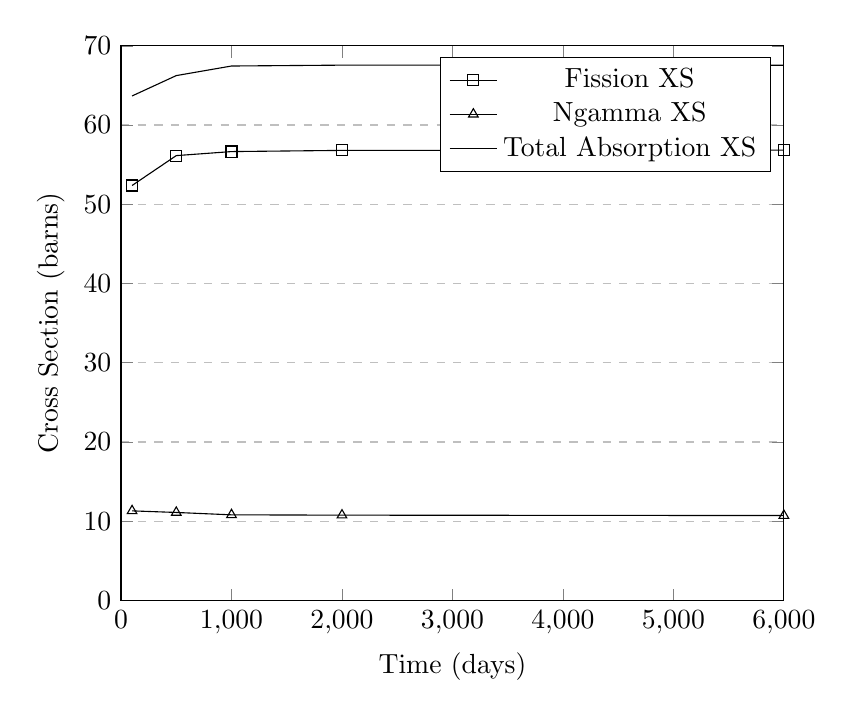
\begin{tikzpicture}
\begin{axis}[
    xlabel={Time (days)},
    ylabel={Cross Section (barns)},
    xmin=0, xmax=6000,
    ymin=0, ymax=70,
    xtick={0,1000, 2000, 3000, 4000, 5000, 6000},
    ytick={0,10,20,30,40,50,60, 70, 80},
    ymajorgrids=true,
    grid style=dashed,
]face

\addplot[
    color=black,
    mark=square,
    ]
    coordinates {
    (100,52.37)(500,56.14)(1000,56.65)(2000,56.80)(6000,56.84)
    };
    \addlegendentry{Fission XS}
\addplot[
    color=black,
    mark=triangle,
    ]
    coordinates {
    (100,11.3)(500,11.1)(1000,10.8)(2000,10.76)(6000,10.71)
    };
    \addlegendentry{Ngamma XS}
\addplot[
    color=black,
    mark=circle,
    ]
    coordinates {
    (100,63.67)(500,66.24)(1000,67.45)(2000,67.56)(6000,67.55)
    };
    \addlegendentry{Total Absorption XS}
\end{axis}
\label{fig:u235xs}
\end{tikzpicture}
\end{figure}

\begin{figure}
\caption{Cross Section Behavior of U238 in 3.5\% enriched LWR. The U238 is subjected to a constant flux of $3x10^14$n/s/$cm^2$.}
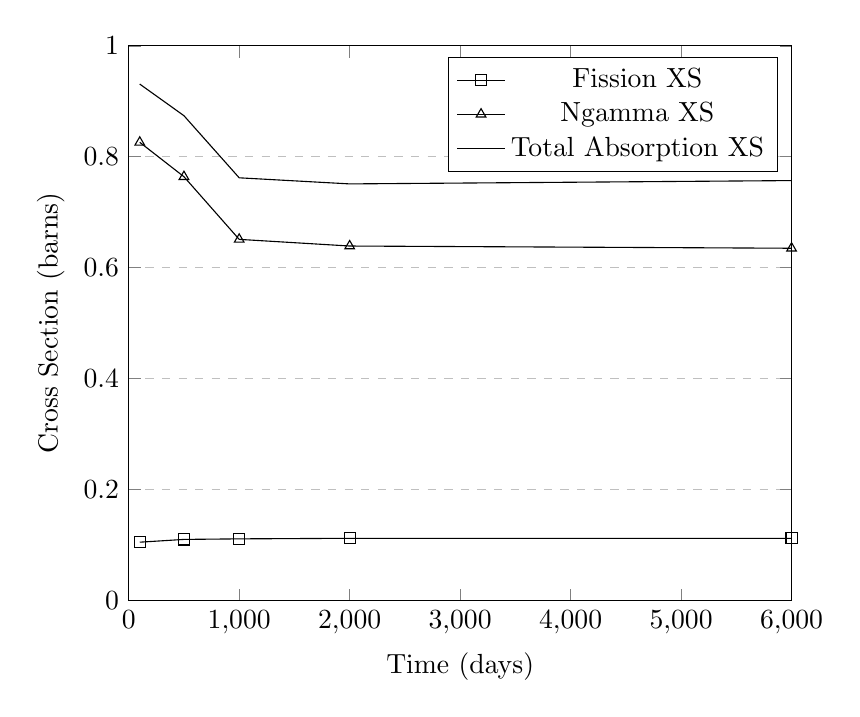
\begin{tikzpicture}
\begin{axis}[
    xlabel={Time (days)},
    ylabel={Cross Section (barns)},
    xmin=0, xmax=6000,
    ymin=0, ymax=1,
    xtick={0,1000, 2000, 3000, 4000, 5000, 6000},
    ytick={0,0.20,0.4,0.6,0.8,1.0},
    ymajorgrids=true,
    grid style=dashed,
]
\addplot[
    color=black,
    mark=square,
    ]
    coordinates {
    (100,0.105)(500,0.11)(1000,0.111)(2000,0.112)(6000,0.112)
    };
    \addlegendentry{Fission XS}
\addplot[
    color=black,
    mark=triangle,
    ]
    coordinates {
    (100,0.826)(500,0.764)(1000,0.651)(2000,0.639)(6000,0.635)
    };
    \addlegendentry{Ngamma XS}
\addplot[
    color=black,
    mark=circle,
    ]
    coordinates {
    (100,0.931)(500,0.874)(1000,0.762)(2000,0.751)(6000,0.757)
    };
    \addlegendentry{Total Absorption XS}
\end{axis}
\label{fig:u238xs}
\end{tikzpicture}
\end{figure}

Figures (\ref{fig:U235xs}, \ref{fig:U238xs}) show how the the fission and ngamma cross sections change slowly over the course of operating the reactor. This is to be expected as the flux and number density of these two isotopes changes. U235 and U238 both undergo a net burn effect, which is why the behavior of the cross sections for these two isotopes change in similar ways over the course of the XSgen simulation. This behavior is consistent with the expected behavior of cross sections within a light water reactor.

Additionally the following figure shows the equalibrium flux of the reactors as determined by OpenMC.
Figure \ref{fig:32g} shows the fluxes of the same XSgen run using two different energy group structures; 32, and 1000.

\begin{figure}[h]
  \center
  \includegraphics[scale=0.7]{fluxes.png}
  \caption{Fluxes generated by OpenMC for a light water reactor using 32 and 1000 group energy structures.}
  \label{fig:32g}
\end{figure}

Figure \ref{fig:32g} shows the expected behavior between the two group structures. The larger group structure manages to catch the effects of some of stronger resonance groups as well as providing better detail to the lower group structures.

\section{LWR Benchmarking Cases}
XSgen by itself can not directly be tested against operating reactor systems. As XSgen is meant to work with medium fidelity reactor models, it will be benchmarked in conjunction with Bright-lite to produce burnups and isotopes for several known reactor systems.  As Bright-lite has already been benchmarked several times using other datasets\cite{brightlite} it is assumed that the operations within Bright-lite are accurate and any deviations within the results come from XSgen.

Primarily the cases represent a range of different enrichments in several light water reactors, comparing the results from XSgen/Bright-lite to recipes from VISION\cite{vision}. Additionally, the values will be tested against two cases modelling reactor startup behavior.

The XSgen/Bright-light will be benchmarked against VISION at 3.0, 3.5, and 4.0 percent enrichment. Three batch cores will be assumed for all the enrichment test cases.
The two cases being used to test XSgen in startup behavior will be a 3.1$\%$ enriched light water reactor using four batches and a 3.6$\%$ enriched light water reactor using four batches. The cases will be compared using burnups, isotopic composition of fresh and used fuel.

\begin{table}[!htb]
\centering
\small
\caption{The output isotopics at equalibrium for the VISION fuel cycle simulator}
\label{tab:a}
\vspace{0.5em}
\begin{tabular}{cccc}
 & \multicolumn{1}{c}{3.0\%} & \multicolumn{1}{c}{3.5\%} & \multicolumn{1}{c}{4.0\%} \\
Nuclide & Mass Fraction & Mass Fraction & Mass Fraction \\
\hline
U235  & 6.75E-3 & 6.80E-3 & 6.95E-3 \\
Pu238 & 1.23E-4 & 1.85E-4 & 2.52E-4 \\
Pu239 & 5.15E-3 & 5.41E-3 & 5.64E-3 \\
Pu240 & 2.38E-3 & 2.60E-3 & 2.78E-3 \\
Pu241 & 1.30E-3 & 1.48E-3 & 1.62E-3 \\
Pu242 & 5.43E-4 & 6.92E-4 & 8.17E-4 \\
Am241 & 3.56E-5 & 4.59E-5 & 5.55E-5 \\
Am243 & 9.38E-5 & 1.37E-4 & 1.76E-4 \\
Cm242 & 1.38E-5 & 1.88E-5 & 2.33E-5 \\
Cm244 & 2.79E-5 & 4.38E-5 & 7.06E-5 \\
\hline
\end{tabular}
\end{table}

\begin{table}[!htb]
\centering
\small
\caption{A comparison of the output isotopics at equalibrium in the VISION fuel cycle simulator and the XSgen-Bright-lite system. Comparison is done as a percent difference.}
\label{tab:xsgenresults}
\vspace{0.5em}
\begin{tabular}{c cc | cc | cc }
 & \multicolumn{2}{c}{3.0\%} & \multicolumn{2}{c}{3.5\%} & \multicolumn{2}{c}{4.0\%} \\
Isotope & Bright-lite & Difference & Bright-lite & Difference & Bright-lite & Difference  \\
\hline
U235 & 6.70E-3 & -0.78 & 6.71E-3 & -1.30 & 6.91E-3 & -0.562 \\
Pu238 & 1.27E-4 & 3.01 & 1.86E-4 & -0.41 & 2.55E-4 & 1.35 \\
Pu239 & 5.25E-3 & 1.95 & 5.45E-3 & 0.66 & 5.67E-3 & 0.57 \\
Pu240 & 2.40E-3 & 0.97 & 2.61E-3 & 0.25 & 2.79E-3 & 0.4 \\
Pu241 & 1.35E-3 & 3.69 & 1.52E-3 & 2.74 & 1.62E-3 & -0.02 \\
Pu242 & 5.48E-4 & 0.88 & 6.93E-4 & 0.10 & 8.19E-4 & -0.28 \\
Am241 & 3.86E-5 & 8.81 & 5.17E-5 & 12.60 & 6.04E-5 & 8.79 \\
Am243 & 9.01E-5 & -3.94 & 1.26E-4 & -7.47 & 1.74E-4 & -1.40 \\
Cm242 & 1.34E-5 & -3.19 & 1.79E-5 & -4.91 & 2.31E-5 & -0.83 \\
Cm244 & 2.57E-5 & -7.94 & 4.54E-5 & -6.06 & 7.00E-5 & -0.90 \\
\hline
\end{tabular}
\end{table}

Table \ref{tab:a} shows the output composition for three different fuel enrichments discussed. These outputs are used as a basis for comparison for Table \ref{tab:xsgenresults}.

Table \ref{tab:xsgenresults} shows a very strong agreement between VISION and Bright-light results using datasets created from light water reactors designed to these particular enrichments. Bright-light has been benchmarked against VISION previously using other datasets. This shows that given XSgen generated datasets allows for Bright-lite to match VISION to a 5\% tolence for a majority of isotopes. Those that exhibit the greatest deviations are high order transuranics.

Am241 shows the largest deviations from the VISION data. There is more Am241 in every case than expected by the VISION results, and less of the species that are arise due to the presence of Am241; Am243, Cm242, Cm244. These results can be explained by a neutron absorption cross section error in Am241. If the neutron absorption cross section for Am241 is too low it can never transmute into Am242 and Am243, which in turn leads to an absence of curium isotopes.

\section{LWR Startup Behavior Benchmarking}
Additionally the Bright-lite model generated by XSgen was tested against a set of Nuclear Enegy Agency (NEA) results\cite{nea}. These results show the start up behavior of the same reaction using two different fuel enrichments.
\begin{table}[!htb]
\centering
\caption{NEA core discharge data for a 3.1\% enriched light water reactor with startup behavior.}
\label{tab:b}
\begin{tabular}{lcccc}
Batch & Burnup (MWd/kg) & U235 (\%) & Fissile Pu (\%) & Total Pu(\%) \\
1 & 12.04 & 0.64 & 0.464 & 0.633 \\
2 & 23.86 & 0.76 & 0.6 & 0.818 \\
3 & 31.75 & 0.8 & 0.677 & 0.921 \\
4 & 32.00 & 0.85 & 0.697 & 0.943 \\
Equil. & 33.00 & 0.85 & 0.688 & 0.943
\end{tabular}
\end{table}

\begin{table}[!htb]
\centering
\caption{The startup values and percent difference from the NEA data for the XSgen/Bright-lite reactor system.}
\label{tab:c}
\begin{tabular}{c cc | cc | cc | cc}
 & \multicolumn{2}{p{1cm}}{Burnup (MWd/kgIHM)} & \multicolumn{2}{c}{U235 (\%)} & \multicolumn{2}{c}{Fissile Pu (\%)} & \multicolumn{2}{c}{Total Pu (\%)} \\
Batch & Value & \%Diff & Value & \%Diff & Value & \%Diff & Value & \%Diff \\
1 & 13.570 & 12.754 & 0.656 & 2.50 & 0.550 & 18.737 & 0.680 & 7.541 \\
2 & 22.040 & -7.628 & 0.723 & -4.868 & 0.641 & 6.919 & 0.835 & 2.189 \\
3 & 32.510 & 2.394 & 0.789 & -1.375 & 0.710 & 4.883 & 0.970 & 5.231 \\
4 & 31.230 & -2.406 & 0.851 & 0.117 & 0.680 & -2.254 & 0.906 & -5.031 \\
5 & 33.010 & 0.030 & 0.843 & -0.824 & 0.703 & 2.198 & 0.946 & 0.285 \\
Equal. & 33.020 & 0.060 & 0.855 & 0.588 & 0.700 & 1.833 & 0.951 & 0.820
\end{tabular}
\end{table}

Table \ref{tab:b} shows how XSgen/Bright-lite compares to the NEA results. The equilibrium results here show good agreement with this case. As Bright-lite is often used to derive output isotopics from used fuels to be passed onto recycle scenarios, accurately predicting the equilibrium discharge is important.

The results of the start up nuclide loading can be seen in Table \ref{tab:c}. The first discrepency in these results is the amount of plutonium generated within the first batch is significantly higher within Bright-lite compared to the NEA data. This trend only continues for the first two cycles. Due to the way Bright-lite operates, this is caused by the lower enriched batches within the startup core that do not have neutron poisons from fission products or other actinides. The high amount of U238 in these initial batches causes a higher production rate of Pu239 over the NEA data. The NEA benchmark has these low enrichment startup batches spread more evenly, Bright-lite simulates them as being the inner most section of the core.

\begin{table}[!htb]
\centering
\caption{NEA data for a 3.6\% enriched light water reactor start up behavior.}
\label{tab:d}
\begin{tabular}{lllll}
Batch & Burnup (MWd/kg) & U235 (\%) & Fissile Pu (\%) & Total Pu(\%) \\
1 & 13.9 & 0.840 & 0.474 & 0.629 \\
2 & 22.67 & 0.721 & 0.642 & 0.892 \\
3 & 32.36 & 0.647 & 0.716 & 1.039 \\
4 & 41.00 & 0.640 & 0.785 & 1.177 \\
5 & 39.00 & 0.940 & 0.808 & 1.166 \\
6 & 40.60 & 0.88 & 0.817 & 1.194 \\
Equil. & 42.50 & 0.81 & 0..827 & 1.223
\end{tabular}
\end{table}

\begin{table}[!htb]
\centering
\caption{XSgen / Bright-lite data for the 3.6\% enriched light water reactor start up behavior.}
\label{tab:e}
\begin{tabular}{l ll | ll | ll | ll}
 & \multicolumn{2}{l}{Burnup (MWd/kgIHM)} & \multicolumn{2}{l}{U235 (\%)} & \multicolumn{2}{l}{Fissile Pu (\%)} & \multicolumn{2}{l}{Total Pu (\%)} \\
Batch & Value & \%Diff & Value & \%Diff & Value & \%Diff & Value & \%Diff \\
1 & 13.37 & -3.84 & 0.930 & 10.77 & 0.62 & 30.43 & 0.78 & 23.53 \\
2 & 22.69 & 0.07 & 0.82 & 13.02 & 0.72 & 12.81 & 0.96 & 7.49 \\
3 & 32.38 & 0.03 & 0.72 & 11.08 & 0.78 & 8.46 & 1.07 & 2.69 \\
4 & 42.57 & 3.83 & 0.61 & -5.33 & 0.804 & 2.42 & 1.14 & -2.94 \\
5 & 41.00 & 5.13 & 0.85 & 9.526 & 0.79 & -2.81 & 1.10 & -5.91 \\
6 & 43.83 & 3.04 & 0.82 & 6.53 & 0.79 & -3.58 & 1.11 & -7.45 \\
Equal. & 42.32 & -0.43 & 0.81 & -0.44 & 0.79 & -4.54 & 1.11 & -9.42
\end{tabular}
\end{table}

Table \ref{tab:d} and Table \ref{tab:e} are repeats of Table \ref{tab:b} and Table \ref{tab:c} for the 3.6$\%$ enriched light water reactor. Again, you see a similar trend in these two with the exception that the equilibrium results for the total amount of plutonium within the reactor is 9.2$\%$ lower in the Bright-lite model. The amount of fissile plutonium is also lower, but within acceptable bounds. The lower amount of fissile plutonium leads to less transmutations into the high order actinides.

\section{MOX Case Benchmarking}
Simply replicating the behavior of a light water reactor would not demonstrate the full capabilities of the XSgen software. To display the capability of the system to extend to more advanced reactor types, XSgen will be used to generate a MOX fuel library for Bright-lite. It will then be used to simulate a single pass MOX reactor. In order to compare this on an apples to apples basis, the input fuel into the Bright-lite reactor will be exactly the same as that for a similar VISION reactor. This test will be able to demonstrate the flexibility of the combined XSgen/Bright-lite system that allows it to model advanced reactor types.

\begin{table}[!htb]
\centering
\caption{Comparison of VISION and Bright-lite result from a single pass MOX reactor.}
\label{tab:g}
\begin{tabular}{lllll}
Nuclide & Input Composition & Vision & Bright-lite & Difference(\%) \\
U234 & 2.20E-4 & 2.11E-4 & 2.00E-4 & -5.0\\
U235 & 7.08E-3 & 4.05E-3 & 4.00E-3 & -1.2\\
U236 & 5.28E-3 & 4.97E-3 & 5.60E-3 & 12.6\\
U238 & 8.80E-1 & 8.51E-1 & 8.62E-1 & 1.3\\
Pu238 & 2.85E-3 & 3.22E-3 & 3.01E-3 & -6.5\\
Pu239 & 5.66E-2 & 3.31E-2 & 3.15E-2 & -4.6\\
Pu240 & 2.70E-2 & 2.42E-2 & 2.54E-2 & 5.0\\
Pu241 & 1.17E-2 & 1.31E-2 & 1.27E-2 & -3.3\\
Pu242 & 8.00E-3 & 8.90E-3 & 8.68E-3 & -2.6\\
Am241 & 1.18E-3 & 1.72E-3 & 1.60E-3 & -7.2\\
Am243 & - & 1.96E-3 & 1.83E-3 & -6.6\\
Cm242 & - & 2.62E-4 & 2.46E-4 & -6.4\\
CM244 & - & 1.03E-3 & 9.84E-4 & -4.4
\end{tabular}
\end{table}

The data in Table \ref{tab:g} shows that the results of Bright-lite given the new XSgen MOX reactor cross section fairs quite well compared to VISION. There are some outliers in the behaviors, specifically the higher order species and U236. The differences with the higher order actinides, Am241 and higher, most likely stem from the high amount of Pu240. This suggests that Pu240 is not transmuting into Pu241 at a high enough rate, which therefore lowers the equilibrium concentration of Pu241 and all isotopes that derive from it.

One of the possible causes of this is uncertainity in the exact dimensions and behavior of the VISION MOX reactor. In order to get the most accurate results XSgen needs to know the specification of the MOX reactor. Instead for this work a generic 17x17 light water reactor core was chosen to use as a base for the XSgen run. If the input and output compositions generated for VISION were made from a reactor core of a different design it would result in slightly different cross sections and therefore different behavior.

\section{Recipe Reactor Generation}
As discussed above, XSgen can be used to create recipe reactors as well. The following results show a comparison between VISION and XSgen recipe reactors. These reactors use a 3.2\% U235 enriched fuel. The XSgen model assumes the information found in Table \ref{tab:xsgenstats} about the reactor.

\begin{table}[!htb]
\centering
\caption{Specification forthe XSgen 33 MWd/kgIHM Burnup LWR.}
\label{tab:xsgenstats}
\begin{tabular}{ll}
Input & Value \\
Fuel Cell Radius & 0.410 cm \\
Void Cell Radius & 0.4185 cm \\
clad Cell Radius & 0.475 cm \\
Unit Cell Pitch  & 1.32 cm \\
Unit Cell Height & 10.0 cm \\
Fuel Density & 10.7 [g/cc] \\
Clad Density & 5.87 [g/cc] \\
Coolant Density & 0.73 [g/cc]
\end{tabular}
\end{table}

Table \ref{tab:recipe} shows the difference between the VISION 3.2\% light water reactor and the XSgen version of that reactor.

\begin{table}[!htb]
\centering
\caption{Comparison of VISION and XSgen for the generation of a 33 MWd/kgIHM Burnup.}
\label{tab:recipe}
\begin{tabular}{llllll}
Isotope & Vision & XSgen & Difference(\%) \\
U235 & 8.06E-03 & 7.84E-03 & -2.85 \\
U238 & 9.44E-01 & 9.67E-01 & 2.36 \\
Pu238 & 1.09E-04 & 1.01E-04 & -7.80 \\
Pu239 & 5.13E-03 & 4.83E-03 & -6.15 \\
Pu240 & 2.25E-03 & 2.41E-03 & 6.52 \\
Pu241 & 1.22E-03 & 1.17E-03 & -4.53 \\
Pu242 & 4.73E-04 & 4.49E-04 & -5.26 \\
Am241 & 2.98E-05 & 2.76E-05 & -7.97 \\
Am243 & 7.90E-05 & 7.23E-05 & -9.31 \\
Cm242 & 1.17E-05 & 1.07E-05 & -9.48 \\
Cm244 & 2.22E-05 & 2.11E-05 & -5.11 \\
\end{tabular}
\end{table}

The results in Table \ref{tab:recipe} show that XSgen is with 10\% error on all output isotopics for this reactor design. A possible cause for this differnce is the method used for extrapolating the data for a multi-batch core from a single batch core. Additionally, the design of the VISION reactor is unknown. This means that the reactor modeled with XSgen may not be a perfect one to one match with the reactor model used for VISION.

\section{Conclusion}
The work of nuclear reactor models is to provide designers and researchers with insight into the behavior of reactors and by extension nuclear fuel cycles. Comparisons between these models is important to understanding how the choice of model might impact the accuracy of the results. Through this work XSgen has demonstrated that it is capable of providing a method of generating one-group cross sections and a number of reactor parameters to be used in benchmark campaigns. This provides a path forward for generating datasets for medium and low fidelity models such that they may all be compared on an equal footing. This will allow researchers to understand how these models affect the results of fuel cycle analysis.

Additionally XSgen provides a method for automating the generation of reactor types for medium fidelity models. The work here linking XSgen to the Bright-lite reactor model shows that XSgen can be used to expand the set of reactor types and reactor designs (i.e. varied burnups, enrichment, or core structure) that Bright-lite has access to. Through this coupling Bright-lite can be used to quickly example fuel cycles with new or interesting reactor technologies.

Future work should aim to expand this coupling to include other medium fidelity models such as CLASS. This will allow for comparisons between medium fidelity models to be performed using the same source for datasets. Additionally, XSgen currently does not have a template for fast reactor designs or accelerator driven systems. If XSgen is going to provide the data for benchmarking campaigns in the future the capability to simulate these reactor technologies are will be necessary.


\bibliography{xsgen}
\bibliographystyle{ieeetr}

\end{document}

